\documentclass{article}

\usepackage[papersize={6cm,6cm},margin=0in]{geometry}
\usepackage{tikz}
\usepackage{pgfplots}
\pgfplotsset{compat=1.17, trig format plots=rad}

\usetikzlibrary{patterns}

\begin{document}

\begin{center}
	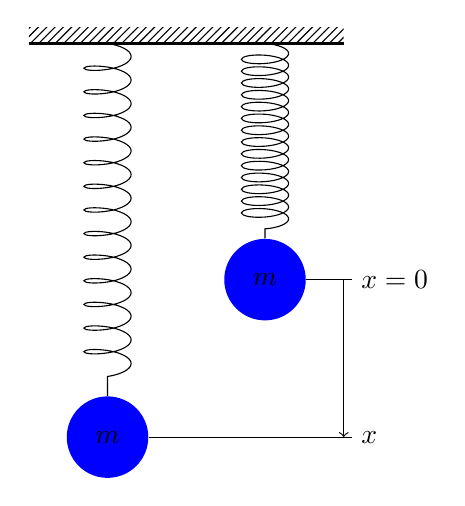
\begin{tikzpicture}
    \node[circle,fill=blue,inner sep=2.5mm] (a) at (0,0) {$m$};
    \node[circle,fill=blue,inner sep=2.5mm] (b) at (2,2) {$m$};
    \draw[decoration={aspect=0.3, segment length=3mm, amplitude=3mm,coil},decorate] (0,5) -- (a); 
    \draw[decoration={aspect=0.3, segment length=1.5mm, amplitude=3mm,coil},decorate] (2,5) -- (b); 
    \fill [pattern = north east lines] (-1,5) rectangle (3,5.2);
    \draw[thick] (-1,5) -- (3,5);
    \draw (b) -- +(1.1,0) node[right]{$x=0$};
    \draw (a) -- +(3.1,0) node[right]{$x$};
    \draw[->] (3,2) -- (3,0) ;
  \end{tikzpicture}
\end{center}
  
\end{document}

